\documentclass[12pt]{article}
\usepackage[a4paper,fancysections,titlepage]{polytechnique}
\usepackage{amsmath,bm,empheq,graphicx,hyperref,siunitx,subcaption,upgreek,xcolor}
\usepackage[italicdiff]{physics}
\usepackage[justification=centering]{caption}

\hypersetup{colorlinks=true, urlcolor=cyan}
\newcommand{\angstrom}{\textup{\AA}}
\newcommand{\ddfrac}[2]{{\displaystyle\frac{\displaystyle #1}{\displaystyle #2}}}

\title{Quantum Criticallity in Cuprate Superconductors: PRL Report}
\author{Matéo Rivera, Saleh Shamloo Ahmadi\\Supervisor: Gaël Grissonnanche}
\date{March 17, 2025}

\begin{document}
\maketitle
\section{Introduction \& Problem Statement}
\subsection{Cuprates: High-Temperature Superconductors}
Cuprates are a class of superconductors with high critical temperature that have been subject
to intense research since their discovery in 1986. They exhibit rich physical behavior, specially
in their various phases.

\begin{figure}
    \centering
    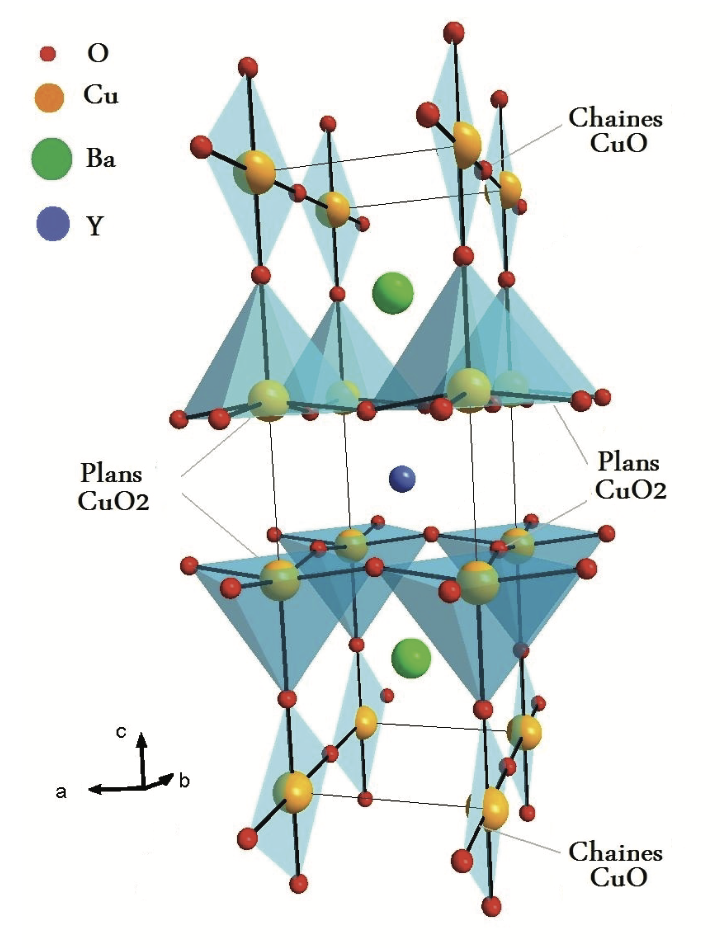
\includegraphics[width=0.5\textwidth]{figures/cuprate_structure}
    \caption{Crystal structure of a Cuprate (YBCO)}
    \label{fig:cuprate_structure}
\end{figure}

The origin of their superconductivity is still a mystery, but it is believed to be related to the
quantum critical point (QCP) that is present in the phase diagram of these materials. The existence
of this QCP is the subject of this research project.

\begin{figure}
    \centering
    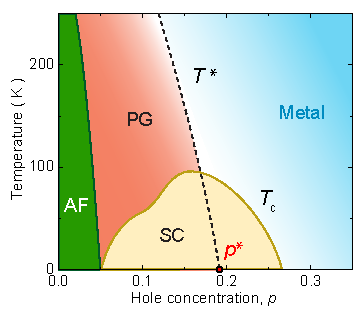
\includegraphics[width=0.5\textwidth]{figures/phase_diagram}
    \caption{Phase diagram of Cuprates. $p^*$ marks the QCP.}
    \label{fig:phase_diagram}
\end{figure}

A quantum critical point is a point in the phase diagram of a material where it goes through a phase
transition at zero temperature. In Cuprates, the phase transition occurs by increasing the doping
level of the material.

\subsection{Evidence for the QCP: Specific Heat}
In their 2019 paper\cite{michon2019}, Michon et al. measured the specific heat of LSCO Cuprates
and found a peak in the specific heat at the critical doping level. This peak is a signature of
the QCP.

\textcolor{red}{TODO: show figure of specific heat vs doping level and discuss the paper in
more detail.}

\subsection{Evidence against the QCP: Optical Conductivity}
In their 2022 paper\cite{legros2022}, Legros et al. measured the optical conductivity of LSCO
Cuprates and, contrary to the specific heat results, found no evidence of a QCP in the optical
conductivity.

To extract the effective mass, they first modeled the conductivity using the Drude formula. This is
a simple classical model that has been used for a long time in condensed matter physics. Then, they
fitted the appropriate formula to the optical conductivity of cuprates in different doping levels.
Finally, they extracted the cyclotron mass from the parameters of the fit. To do so, they calculated
the cyclotron frequency in different magnetic fields and found the mass by fitting a linear relation
between the cyclotron frequency and the magnetic field;
\begin{equation}
    \omega_c = \frac{eB}{m_c}.
\end{equation}
They argue the cyclotron mass is the same as the effective mass of the charge carriers
($m_c \sim m^*$), which is itself proportional to the specific heat and is expected to diverge at
the QCP. They found a simple linear dependence of the cyclotron mass with the doping level, which
contradicts the specific heat results.

We believe, however, that their data analysis is problematic, because of the use of the Drude
formula. Eventhough the Drude formula is derived using classical physics, it is highly effective for
analysing the conductivity of materials, which emerges from the collective quantum behavior of the
electrons. However, this is only the case when the Fermi surface is roughly isotropic (i.e. when the
crystal structure does not exhibit high anisotropy), which is not true for Cuprates, which have a
highly anisotropic Fermi surface. Also, the effective mass of the charge carriers is not necessarily
the same as the cyclotron mass, but we only focus on the former issue in this project.

\textcolor{red}{TODO: show the results of Legros et al. in a figure}

\section{Methods}
\textcolor{red}{COMMENT: This section is, inescapably, a bit technical. Maybe we should warn the
reader? I'm not sure.}

To decisively refute the results of Legros et al., we first reproduced their results (to make sure
there were no errors in their data analysis), then we used a more sophisticated model called
Boltzmann trasport (Chambers formula in the context of conductivity), which can handle anisotropic
Fermi surfaces, to redo the analysis.

\subsection{Reproduction of Drude Fits}
Following Legros et al.\cite{legros2022} and others\cite{post2021}, to fit the optical conductivity,
we use the two-component Drude model with normal and superconducting carriers. The complex optical
conductivity in the left/right circular polarization basis is given by
\begin{equation}
    \sigma_{ll/rr}(\omega) = i\epsilon_0\qty(
        \frac{\omega^2_{\mathrm{p,n}}}{\omega-\omega_c+i\Gamma}
        + \frac{\omega^2_{\mathrm{p,s}}}{\omega} - \omega(\epsilon_{\infty} - 1)),
\end{equation}
where $\omega$ is the frequency of the electromagnetic waves and the adjustable parameters are
\begin{itemize}
    \item $\omega_{\mathrm{p,n}}$ and $\omega_{\mathrm{p,s}}$: plasma frequencies of the normal and
        superconducting carriers,
    \item $\omega_c$: cyclotron frequency,
    \item $\Gamma$: scattering rate,
    \item $\epsilon_{\infty}$: high-frequency dielectric constant.
\end{itemize}
Left handed circular polarization is given by a negative omega and right handed by a positive omega.

As stated in Legros et al. and other sources, the high-frequency dielectric constant does not
greatly improve the quality of the fit and its results, so it is set to 1.

To perform the fit, we used a simple least-squares method, since the optimization is
mostly convex.

Since the raw data of Legros et al. is not publicly available, we digitized the data from their
paper using a custom script extracting the data from svg exports of the figures.

\subsection{Bolzmann Transport and Chambers Formula for Optical Conductivity}
The Boltzmann transport equation is a semi-classical model of flow. Using it, with a few reasonable
assumptions, one can derive the Chambers formula for conductivity. The formula is usually applied
for DC resistivity, but it can be generalized for optical conductivity.

This model has been used successfully to study the behavior of cuprates and make predictions about
their physical properties\cite{grissonnanche2021}.

According to the Chambers formula for optical conductivity, the conductivity tensor in the cartesian
basis is given by
\begin{equation}
	\sigma_{ab} = \frac{2e^2}{(2\pi)^d\hbar}\int_{FS}\dd{\vb{k}}\hat{v}_a(\vb{k})
        \int_0^{\infty}\dd{s}v_b(\vb{k}(s))\exp{i\omega s
        - \int_0^s \frac{\mathop{ds'}}{\tau(\vb{k}(s'))}}
\end{equation}
where $FS$ is the Fermi surface, $d$ is the number of dimensions of the system, $\vb{k}$ is the
wavevector, $\omega$ is the frequency of the electromagnetic waves, $v_b$ is the veclocity of the
charge carriers in the $b$ direction, $\hat{v}_a\equiv v_a/\abs{\vb{v}}$, and $\tau$ is the
relaxation time (inverse of the scattering rate). In order to evaluate the integral, we should
couple this with
\begin{enumerate}
    \item the movement equation,
    \item a model for the scattering rate, and
    \item the shape of the Fermi surface.
\end{enumerate}

As you can see, the Chambers formula contains a lot more information about the electronic structure
of the material, which can show more subtleties in the physical description of the material.
In the following, we explain in more detail the different components and the methods of evaluating
this formula.

\subsubsection{Movement Equation}
Since we are only interested in the first order response of the system to an electric field, we
can solve the movement equation with only a magnetic field. That is,
\begin{empheq}[left=\empheqlbrace]{align}
    \hbar\dv{\vb{k}}{t} &= e\vb{v}\times\vb{B}, \\
    \vb{v} &= \frac{1}{\hbar}\grad_{\vb{k}}\varepsilon(\vb{k}),
\end{empheq}
Where $\varepsilon$ is the energy of the charge carriers. The movement equation can be solved
numerically for a discretization of the Fermi surface (since the Chambers formula integral is
evaluated over the Fermi surface).

\subsubsection{Scattering Rate}
Following Grissonnanche et al.\cite{grissonnanche2021}, we used a simple model for the scattering
rate, respecting the symmetry of the system. It is given by
\begin{equation}
    \frac{1}{\tau(\vb{k})} = \Gamma(\vb{k}) = \Gamma_0 + \Gamma_k\abs{\cos(2\varphi)}^\nu,
\end{equation}
where $\varphi$ is the angle between the wavevector and the $k_x$ axis and $\Gamma_0$, $\Gamma_k$,
and $\nu$ are adjustable parameters.

\subsubsection{Fermi Surface}
For the shape of the Fermi surface, we used a simple 3D tight-binding model for the Body centered
tetragonal crystal structure of LSCO, given by
\begin{equation}
\begin{aligned}
    \varepsilon(\vb{k}) = &-\mu - 2t(\cos(k_x a) + \cos(k_y a)) \\
        &- 4t'\cos(k_x a)\cos(k_y a) - 2t''(\cos(2k_x a) + \cos(2k_y a)) \\
        &- 2t_z\cos(k_x a / 2)\cos(k_y a / 2)\cos(k_z c / 2)[\cos(k_x a) - \cos(k_y a)]^2,
\end{aligned}
\end{equation}
where $\mu$ is the chemical potential, $t$, $t'$, and $t''$ are the first, second, and third
nearest-neighbor hopping parameters, $t_z$ is the interlayer hopping parameter,
$a=\si{3.75}{\angstrom}$ is the in-plane lattice constant, and $c/2=\si{6.6}{\angstrom}$ is the
$\mathrm{CuO_2}$ layer spacing.

\subsubsection{Numerical Calculation of the Conductivity}
\begin{figure}
    \centering
    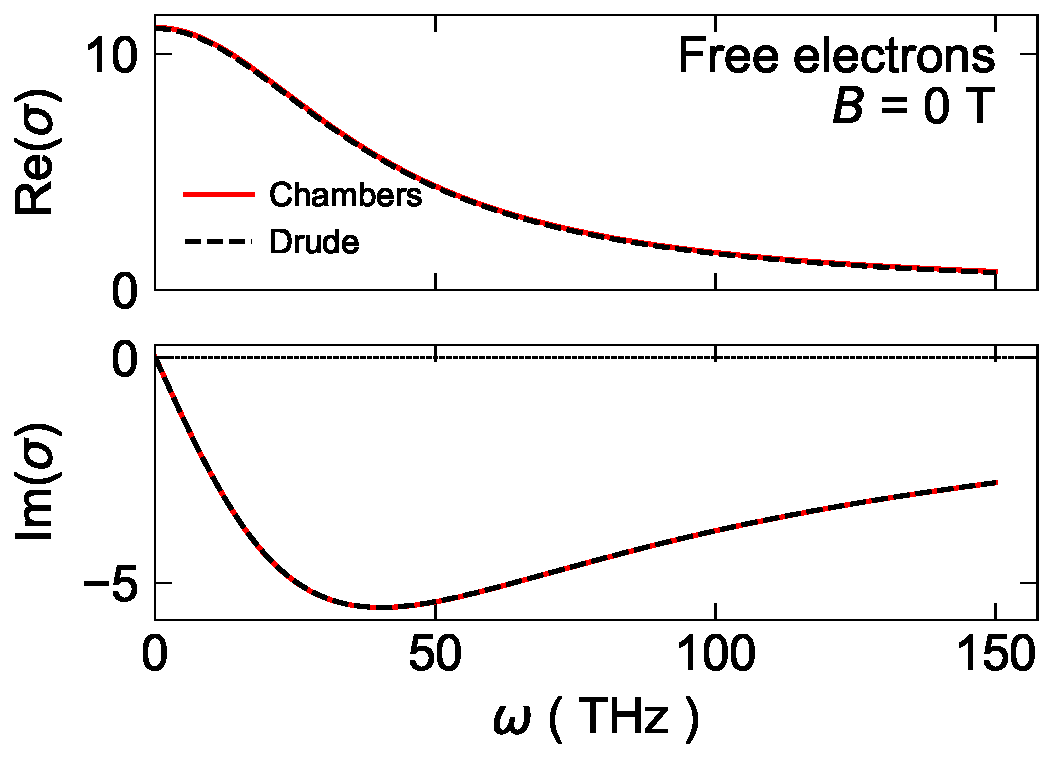
\includegraphics[width=0.7\textwidth]{figures/free_electrons}
    \caption{Fermi surface of LSCO}
    \label{fig:free_electrons}
\end{figure}

\begin{figure}
    \centering
    \begin{subfigure}{0.495\textwidth}
        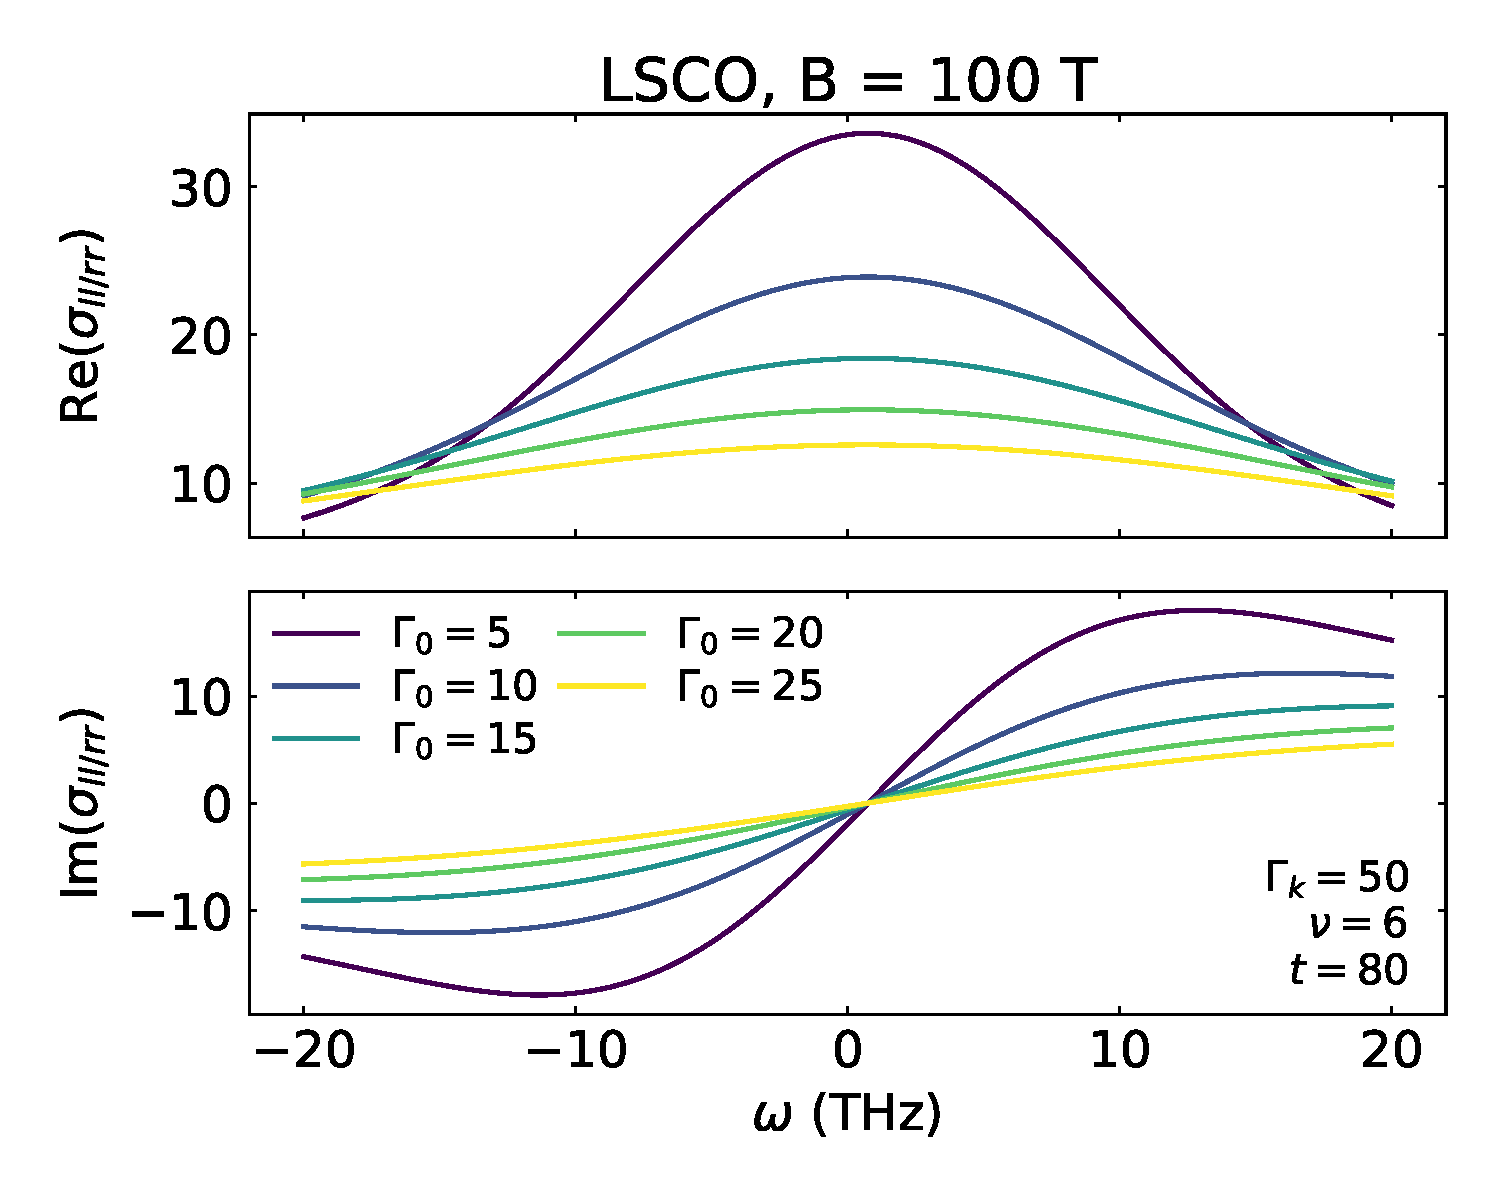
\includegraphics[width=\textwidth]{figures/vary_gamma_0}
        \caption{Varying the isotropic scattering rate}
    \end{subfigure}
    \begin{subfigure}{0.495\textwidth}
        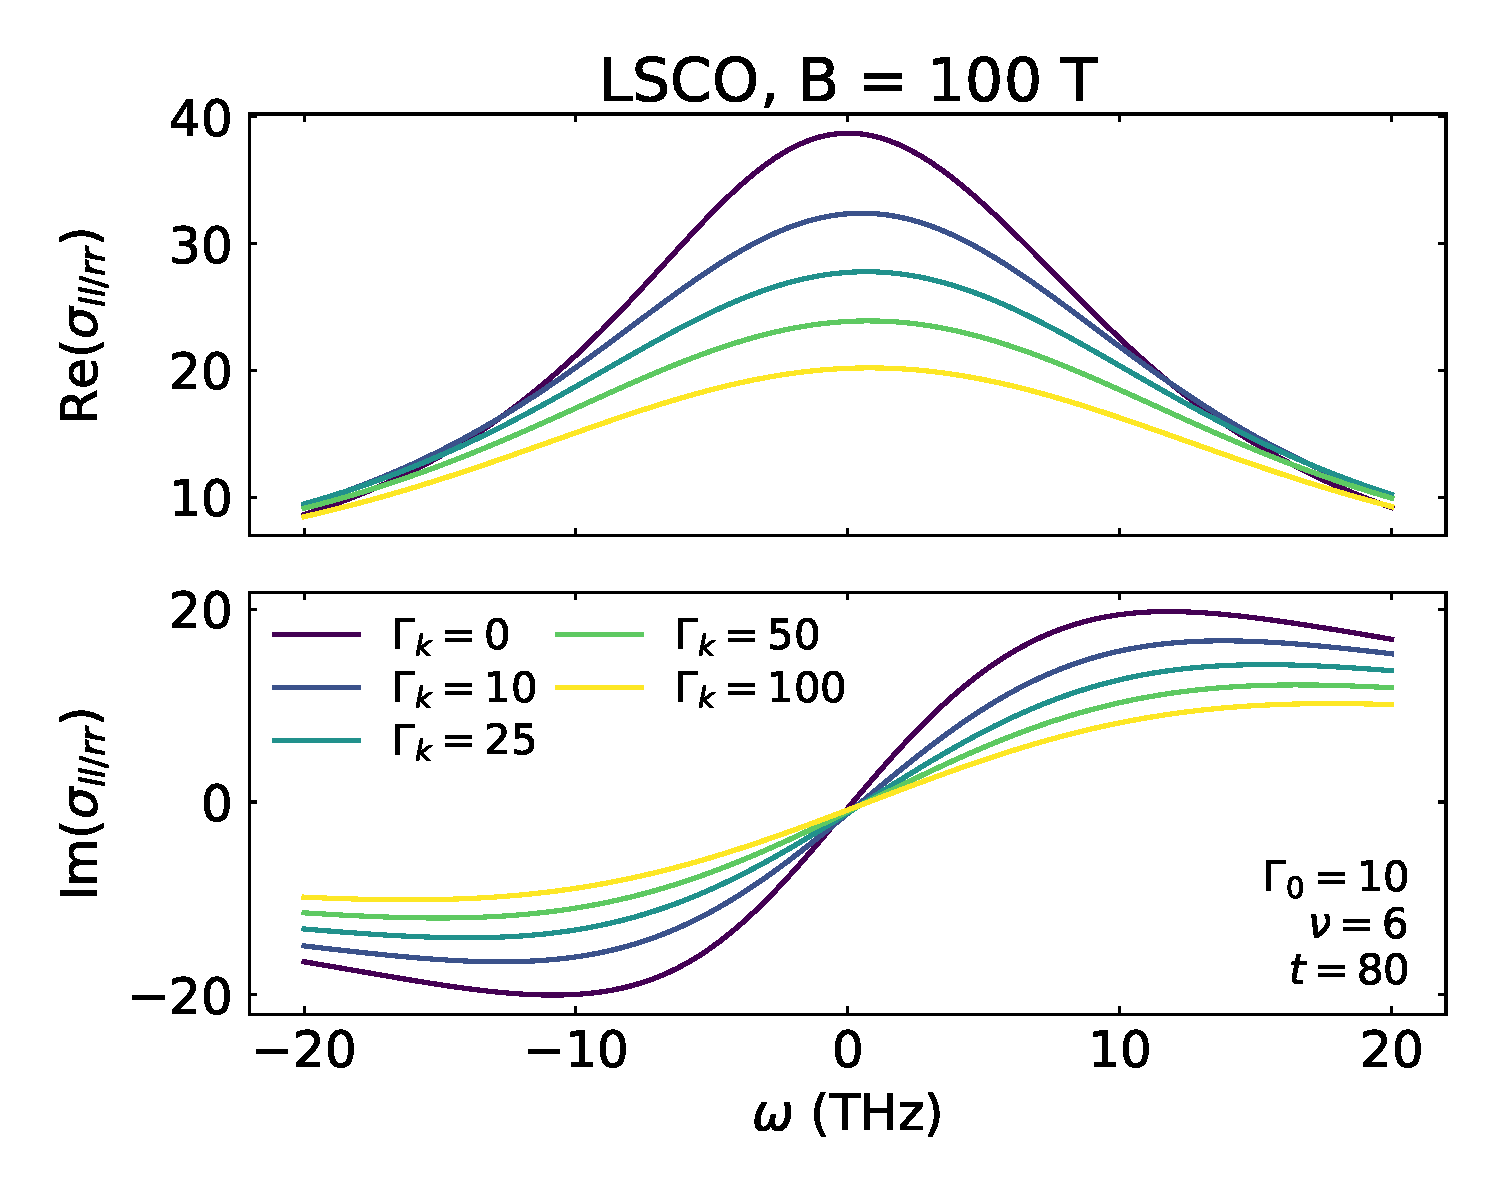
\includegraphics[width=\textwidth]{figures/vary_gamma_k}
        \caption{Varying the anisotropic scattering coefficient}
    \end{subfigure}
    \begin{subfigure}{0.495\textwidth}
        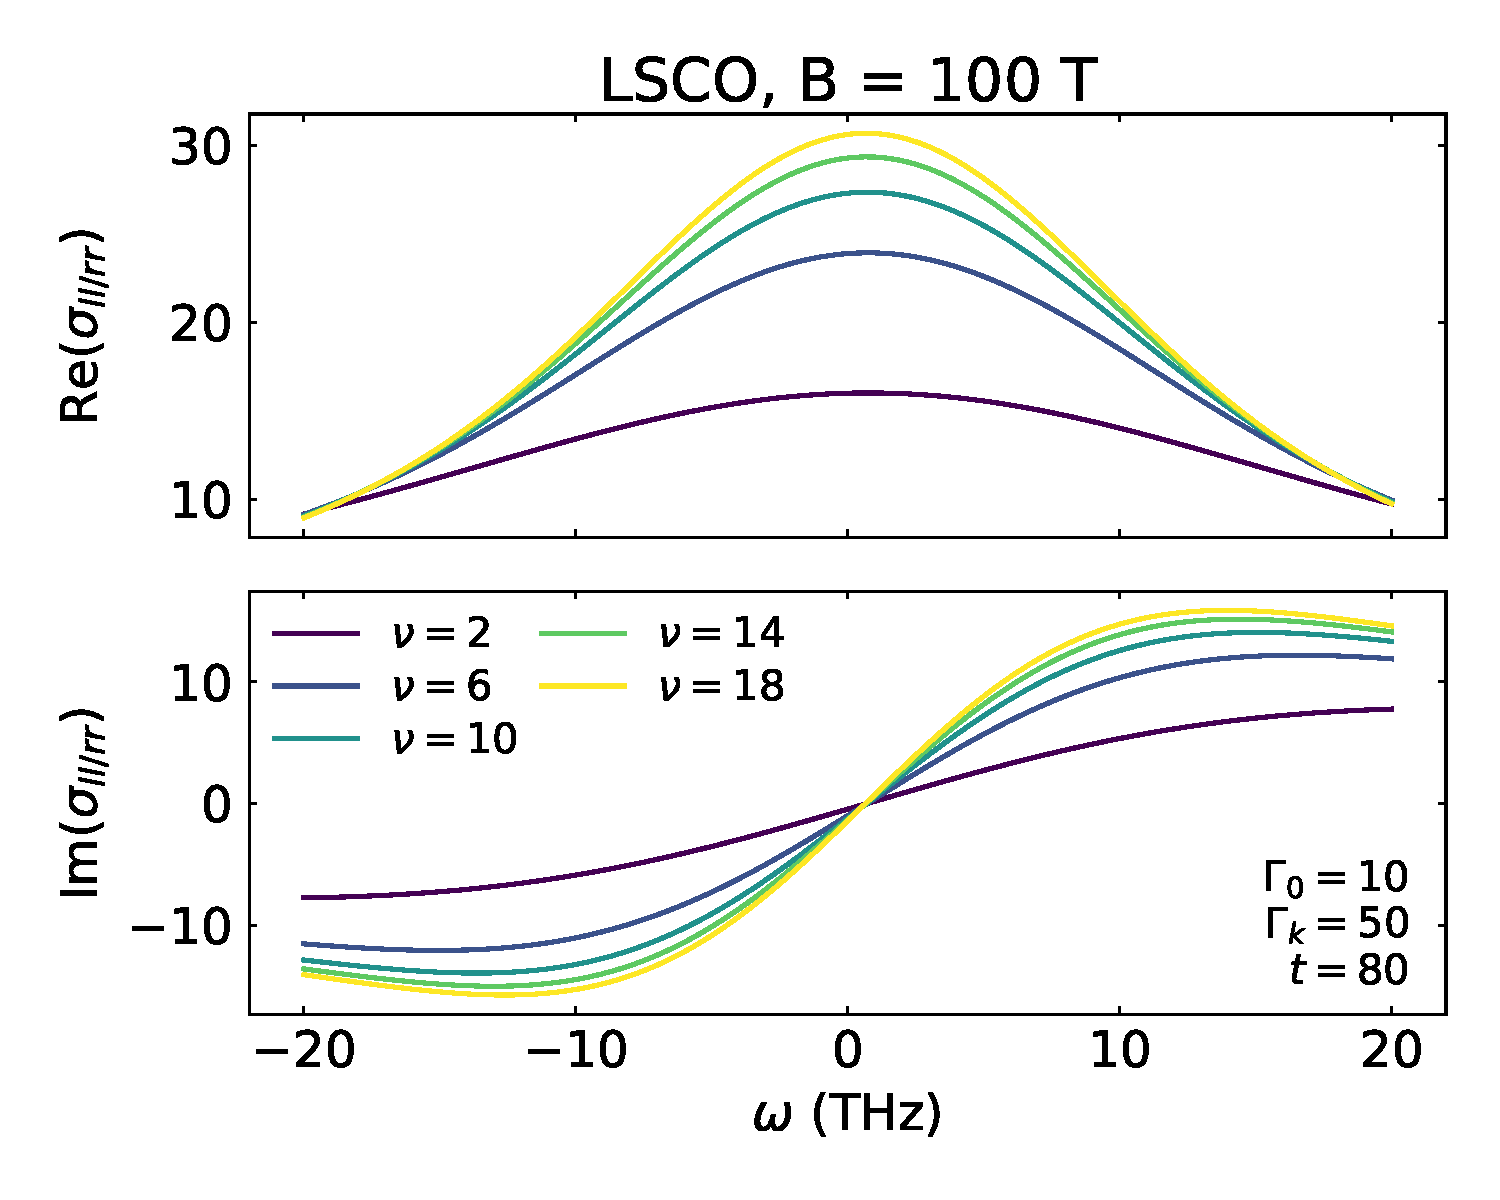
\includegraphics[width=\textwidth]{figures/vary_power}
        \caption{Varying the anisotropic scattering exponent}
    \end{subfigure}
    \begin{subfigure}{0.495\textwidth}
        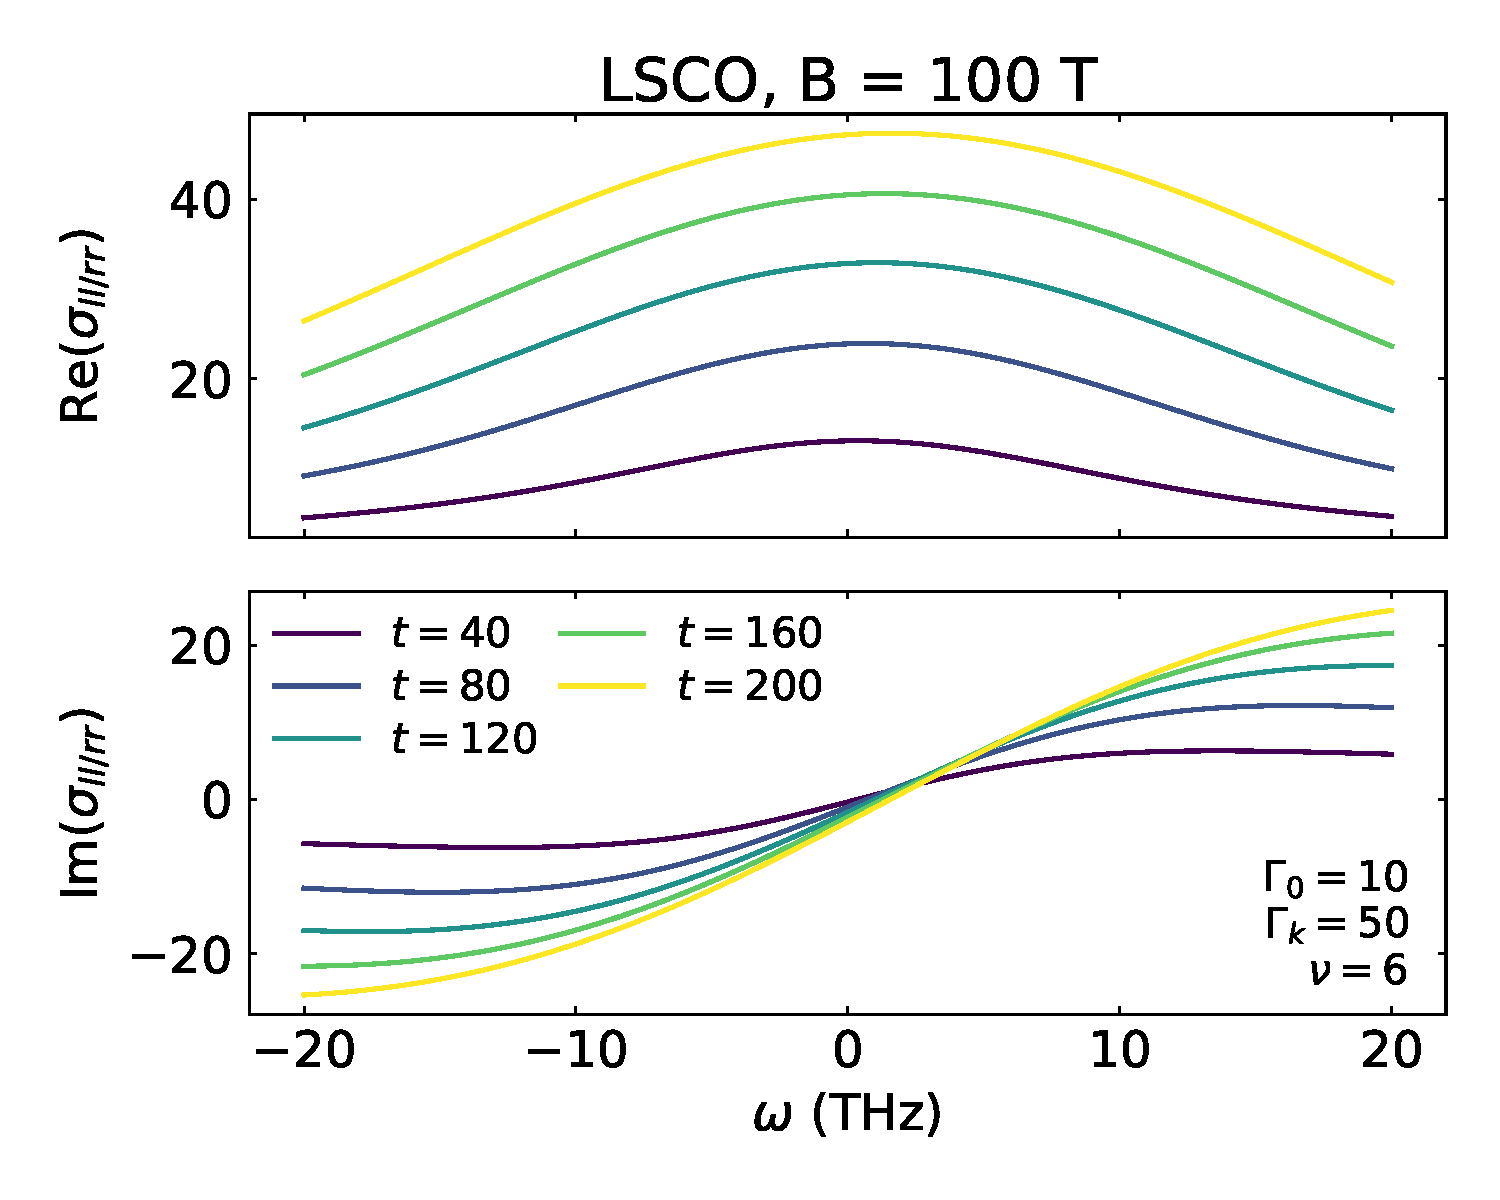
\includegraphics[width=\textwidth]{figures/vary_energy_scale}
        \caption{Varying the energy scale}
        
    \end{subfigure}
    \caption{Effect of varying different model parameters}
    \label{fig:vary_parameters}
\end{figure}

\begin{figure}
    \centering
    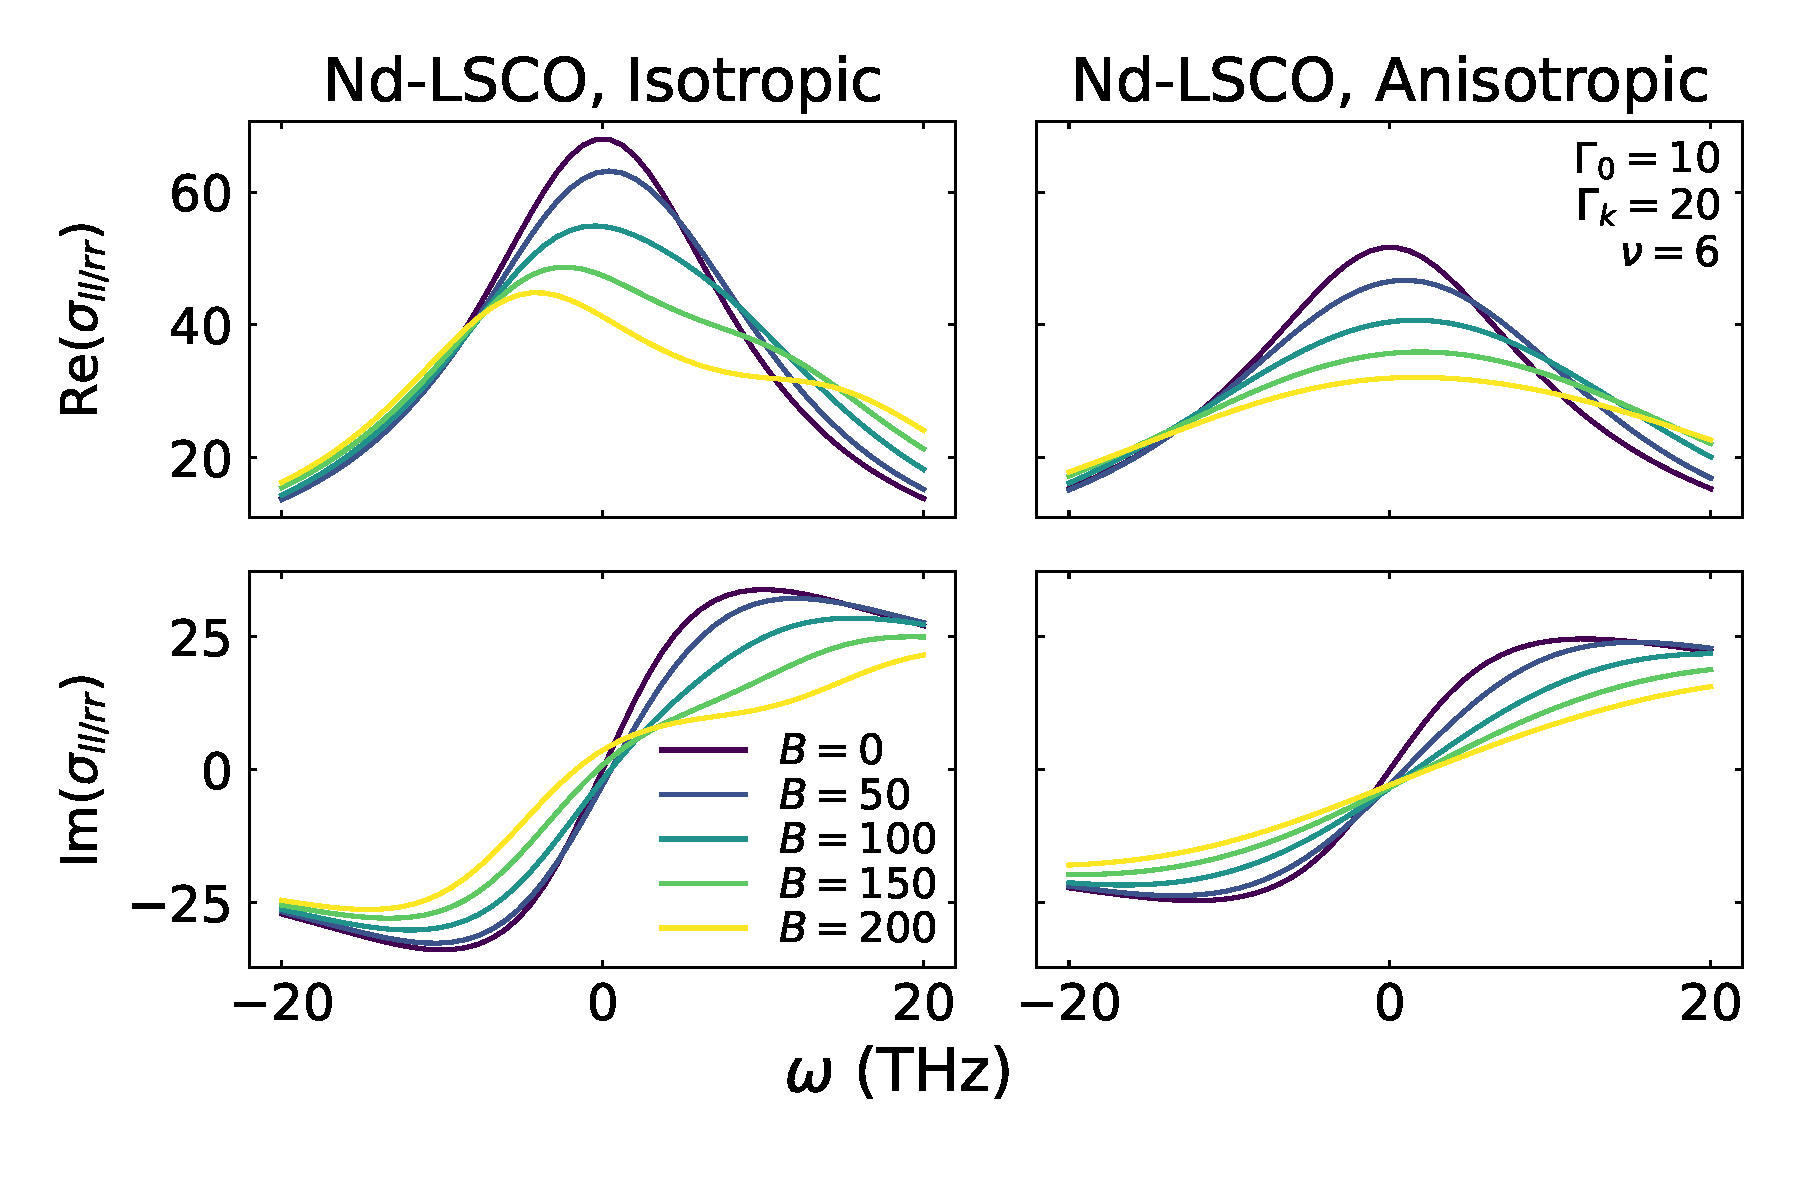
\includegraphics[width=0.7\textwidth]{figures/vary_field}
    \caption{Varying the magnetic field}
    \label{fig:vary_field}
\end{figure}

Grissonnanche et al. have developed a package in Python implementing the Boltzmann transport model.
We first generalized the calculations in this package from (real valued) DC resistivity to (complex
valued) optical conductivity. To check our results, we compared the output of our model to the Drude
model for free electrons (Figure \ref{fig:free_electrons}), since the Chambers formula and the Drude
formula should be equivalent in this case. We then explored how the different parameters affect the
conductivity to get a feel for the model before fitting it to the data.

Looking at the effect of the different parameters in Figure, it seems each parameter roughly has
these effects:
\begin{itemize}
    \item Isotropic scattering rate ($\Gamma_0$): affects the overall magnitude of the conductivity
        and the width of the real conductivity peak.
    \item Anisotropic scattering coefficient ($\Gamma_k$): mostly affects the magnitude of the
        conductivity.
    \item Anisotropic scattering exponent ($\nu$): affects the shape of the real conductivity peak
        and greatly affects the magnitude of the conductivity.
    \item Energy scale: affects the magnitude of the conductivity and the position of the real
        conductivity peak, which means it affects the response of the peak to the magnetic field.
\end{itemize}

Figure \ref{fig:vary_field} shows the exagerated effect of the magnetic field on the conductivity.
Because the Fermi surface of LSCO has electron-like and hole-like regions, a model with no
anisotropic scattering would have two conductivity peaks, one for each type of charge carrier. The
anisotropic scattering would kill one of the peaks, because the electron-like region in
LSCO's Fermi surface has far more anisotropy (i.e. curvature) than the hole-like region.

\textcolor{red}{TODO: add Fermi surface plot of LSCO}

\subsection{Fitting Procedure}
The Boltzmann transport model is way more complex than the Drude model, and can have a non-convex
optimization landscape. So we used a more sophisticated global optimization algorithm, called
differential evolution.

The tight-binding model for the Fermi surface of LSCO has already been studied by other, so we just
used the parameters from the literature. The adjustable parameters are the scattering model
parameters and the energy scale,  which is a scaling factor for the tight binding parameters,
defined as the value of $t$. The other tight binding parameters ($t'$, $t''$, and $t_z$) are defined
as multiples of $t$.

We have data for different doping levels and different magnetic fields. A naïve approach would be to
fit the data for each doping level and each magnetic field separately. However, since the data does
not exhibit a complex behavior, fitting only to one curve at a time would not constrain the
paarameters enough and would lead to overfitting (due to an ill-defined optimization landscape). So,
we fit multiple magnetic fields for each doping level simultaneously. To make sure our fit makes
sense, we redo the fit for different sets of magnetic fields and compare the fitting parameters.
If they are consistent, we can be confident in the results.

\section{Results}
\subsection{Reproduction of Drude Fits}
We could reproduce most of the results of Legros et al. (Figure \ref{fig:drude_fit_good}).
However, no matter how much we fine-tuned the fitting procedure, we could not produce fits looking
as good as theirs for some of the plots (Figure \ref{fig:drude_fit_bad}). So, we tried fitting the
real part and the imaginary part of the optical conductivity separately, and we could produce
similar-looking fits. Extracting the parameters from these fits and comparing them to the parameters
extracted from the fits of Legros et al., we found that the parameters were consistent. This leads
us to believe this is indeed what Legros et al. did in their analysis. This is not ``correct'' in
some sense, but since the imaginary part of the optical conductivity is dominated by a
superconducting singularity, fitting it separately is a reasonable choice.

\begin{figure}
    \centering
    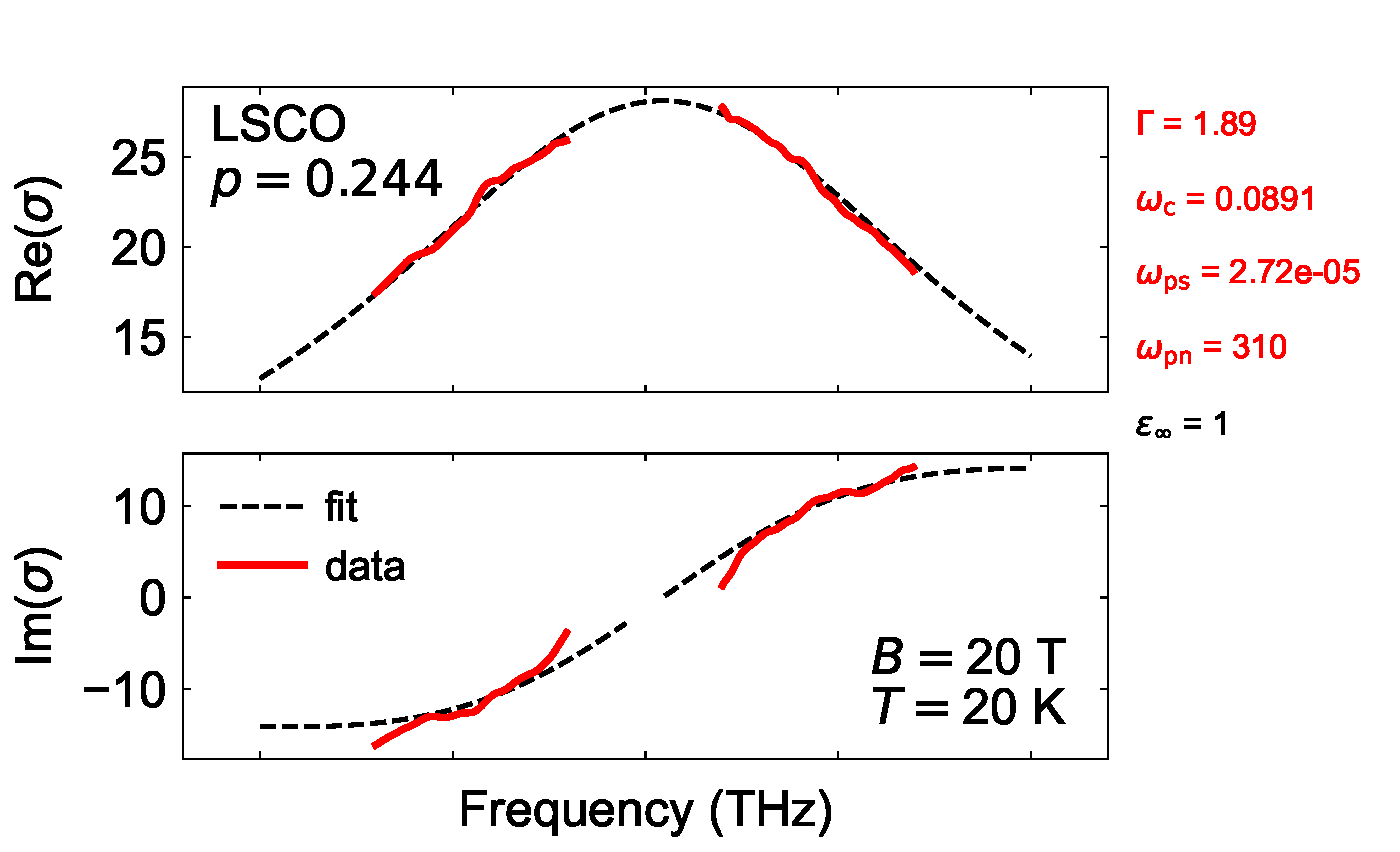
\includegraphics[width=0.7\textwidth]{figures/drude_fit_good.pdf}
    \caption{A good fit while fitting the real and imaginary parts of the optical conductivity
        simultaneously.}
    \label{fig:drude_fit_good}
\end{figure}
\begin{figure}
    \centering
    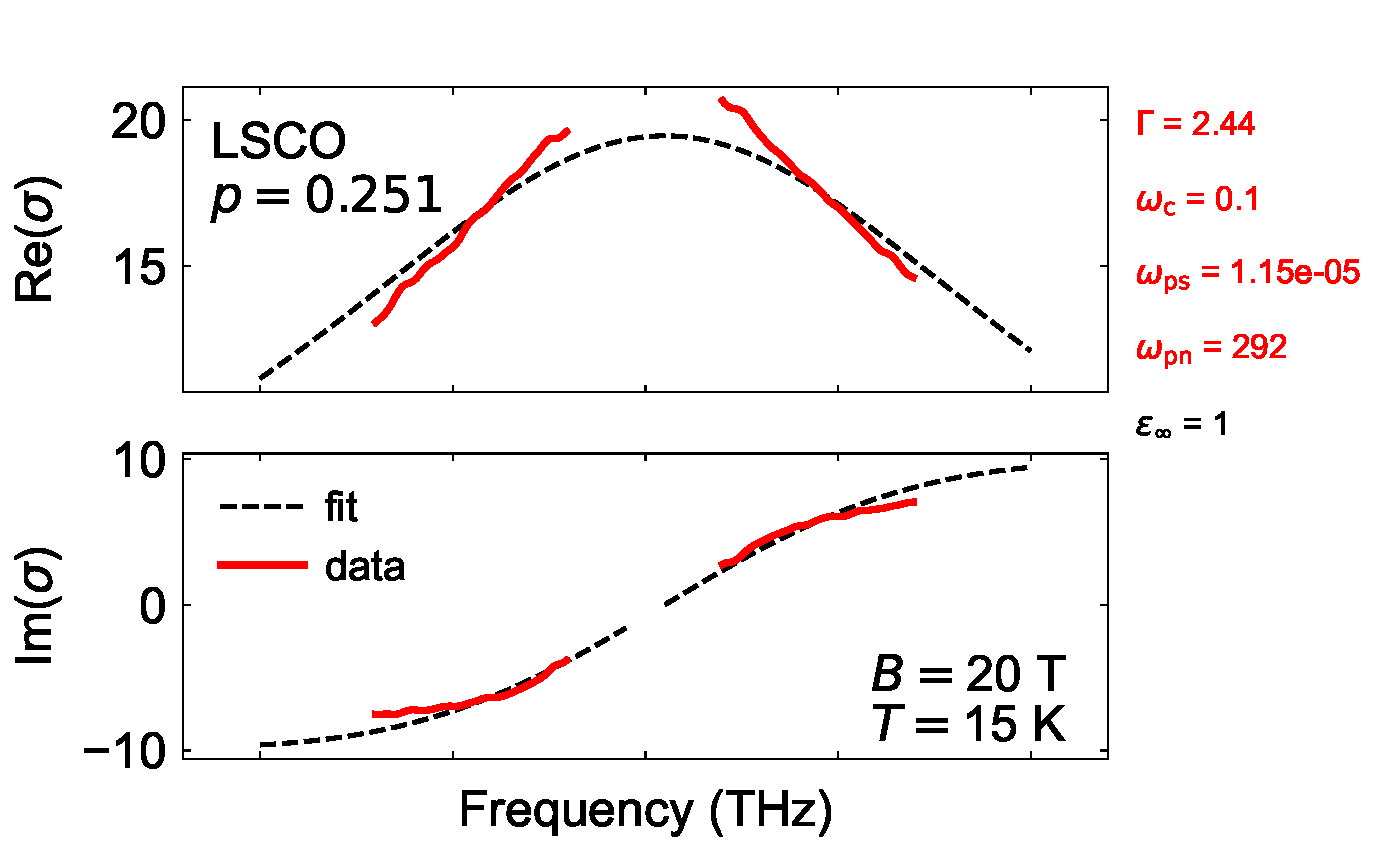
\includegraphics[width=0.7\textwidth]{figures/drude_fit_bad.pdf}
    \caption{A bad fit while fitting the real and imaginary parts of the optical conductivity
        simultaneously.}
    \label{fig:drude_fit_bad}
\end{figure}
\textcolor{red}{TODO: add a figure only fitting to the real part}

\subsection{Boltzmann Transport Fits}
\textcolor{red}{TODO}
\subsection{Discussion}
\textcolor{red}{TODO}\\\\
\textcolor{red}{TODO: write appendices for deriving the Chambers formula and showing the equivalence
to the Drude model in the case of free electrons.}

\bibliographystyle{plain}
\bibliography{ref}

\end{document}
